% Chapter Template

\chapter{Literature Review} % Main chapter title

\label{Chapter2} % Change X to a consecutive number; for referencing this chapter elsewhere, use \ref{ChapterX}

\lhead{Chapter 2. \emph{Literature Review}} % Change X to a consecutive number; this is for the header on each page - perhaps a shortened title

%----------------------------------------------------------------------------------------
%	SECTION 1
%----------------------------------------------------------------------------------------

\section{Introduction}
%\begin{figure}[h]
%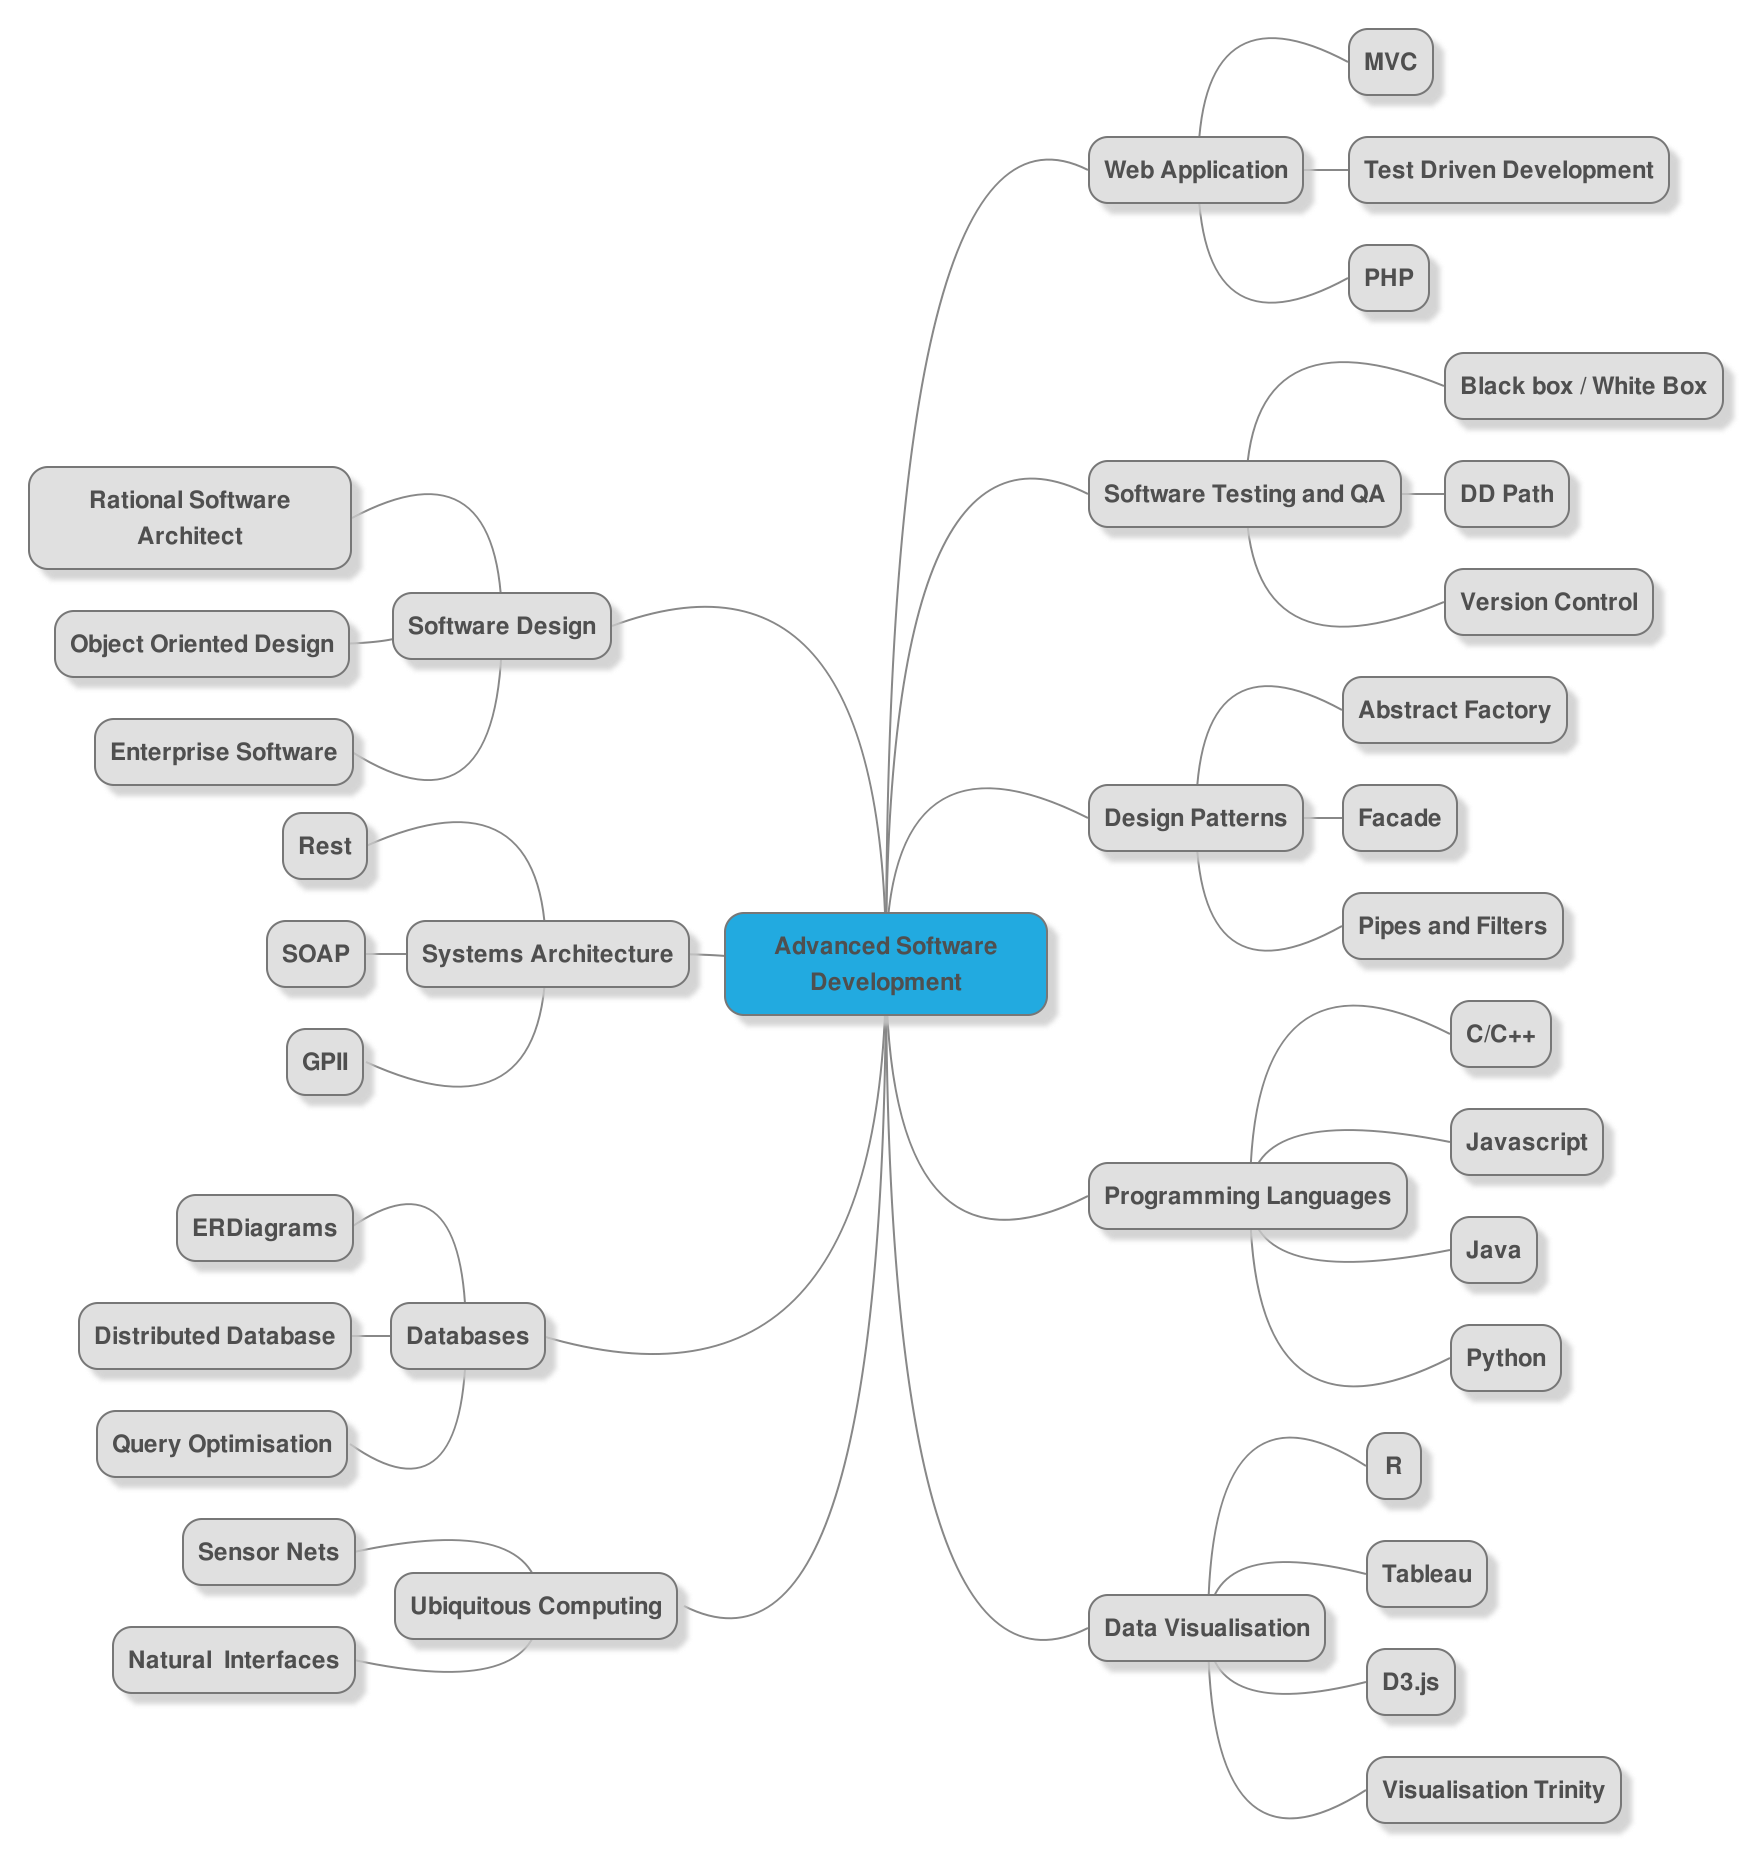
\includegraphics[scale=.2]{mindmap}
%\caption{A mind map of my discipline}
%\centering
%\end{figure}
%-----------------------------------
%	MACHINE LEARNING
%-----------------------------------
\section{Machine Learning}

Mitchell (2006) defines machine learning as a field of computer science that attempts to solve the question:

“How can we build computer systems that automatically improve with experience, and what
are the fundamental laws that govern all learning processes?”

Mitchell outlines that while there had been no successful commercial applications of machine learning as late as 1985, it has since been successfully applied in diverse fields such as speech recognition, computer vision, bio-surveillance, robot control and accelerating empirical sciences.

The literature makes the distinction between different learning scenarios. Alpaydin (2004) explains that ‘supervised learning’ happens in a scenario in which the task of the algorithm is to learn the mapping from some input X to an output Y. Examples of supervised learning problems include regression and classification. This could be contrasted with unsupervised learning; described by Mohri, Rostamizadeh and Talwalkar (2012) as problems in which “the learner receives unlabelled training data and makes predictions for all unseen points.” Examples of supervised learning problems include clustering and dimensionality reduction.
Also reinforcement learning.


\section{Supervised Learning}

Kotsiantis\cite{kotsiantis2007supervised} provides a review of supervised learning classification techniques. "known labels (the corresponding correct outputs) then the learning is called supervised"


Ng (2000) explains that supervised learning algorithms can be divided in regression problems (when the output to be predicted is continuous) and classification problems (when the output to be predicted is discrete). Linear and logistic regression are two machine learning techniques for solving these kinds of supervised learning problems.

\subsection{Regression}

Linear Regression
Non-Linear Regression
Logistic Regression
Regularisation

\subsection{Decision Tables}

Kohavi (1995) proposed decisions tables as a representation for hypothesis in order to solve supervised machine learning problems.
Kohavi provides a comparison of machine learning techniques.
In the absence of an expert data must be collected in a brute force fashion. Problems: noise, missing values, irrelevant input features.
"Once preliminary testing is judged to be satisfactory the classifier (mapping from unlabeled instances to classes) is available for routine use"
"Three techniques to assess accuracy: split training set, cross fold validation, leave-one-out validation".

Logic Based Algorithms  - Decision Trees, Rule based classifiers

Perceptron-Based Algorithms - Neural Networks

Statistical Learning Algorithms - Baysian Networks

Support Vector MAchines

\subsection{Bayesian Networks}

Jensen (1996) explains that Bayesian Networks provide methods for dealing with uncertainty by graphically modelling causal relationships.

\subsection{Artificial Neural Networks}

The state of the art in machine learning is “deep” learning, currently being utilised by Google, Microsoft, IBM and others. Arel, Rose and Karnowski (2010) outline how deep learning overcomes the exponential growth in learning complexity associated with an increase in data dimensionality. Deep learning focuses on the development of computational models that represent information in a fashion similar to the neocortex. Convolutional Neural Networks are described as being the first successful approach to learning many dimensions in a complex manner. Deep belief networks are “probabilistic generative models”; provide a different solution to the problem of deep learning by providing probabilities associated with observations and labels bidirectionally.

\subsection{Decision Tree Learning}

Murthy\cite{murthy1998automatic} decision trees

\subsection{Support Vector Machines}

\section{Unsupervised Learning}

Unlabeled data (no corresponding correct outputs)

\subsection{Clustering}

\subsection{K-means}

%-----------------------------------
%	ARGUMENTATION THEORY
%-----------------------------------

\section{Argumentation Theory}

\subsection{Non-Monotonic Reasoning}


Reiter (1980) recognised the need to make assumptions when presented with incomplete evidence and proposed a logic for default reasoning. Default reasoning is a formalisation of what we believe to be true in the absence of other evidence that makes the case exceptional.
Take the example “Tweety is a bird, birds can fly, therefore Tweety can fly.” Tweety being able to fly is inferred by default since Tweety is a bird. If Tweety is a penguin, on the other hand, Tweety cannot fly. Reiter descibed default reasoning as non-monotonic. In first order logic arguments are monotonic, i.e. what they infer doesn’t change in the presence of new evidence. In the example just given, Tweety can still fly even if he is a penguin. Since default logic is non-monotonic if recognises the need to revise beliefs in the face of new evidence.

thigns
\subsection{Defeasible Reasoning}

Pollock (1987) recognised that while non-monotonic logic in AI is similar to how humans reason, it was also falling short in it’s recognition of the complexities of reasoning. Pollock defined a proposition as being warranted if it would be believed by an ideal reasoner. Reasoning can be said to be defeasible if the premises taken in isolation can infer a conclusion, but that this conclusion can be defeated when additional information is added. Pollock argued that defeasible reasoning (taken from philosophy) more accurately modelled argumentation than AI's non-monotonic reasoning, which he described as simplistic. He also described the usefulness of constructing computer programs to test the accuracy of philosophical models of reasoning.


\subsection{Argumentation Theory in AI}

Dung (1993) was concerned with modelling the fundamental mechanism humans use to argue so as to implement this model on computers. He summarised the basis for his work in the old saying “the one who has the last word laughs best.” In other words, in human typical human argumentation the last piece of evidence to be produced can nullify evidence produced earlier by opposing arguments winning the argument.

\begin{figure}[h]
\caption{Example of an argumentation framework}
\centering
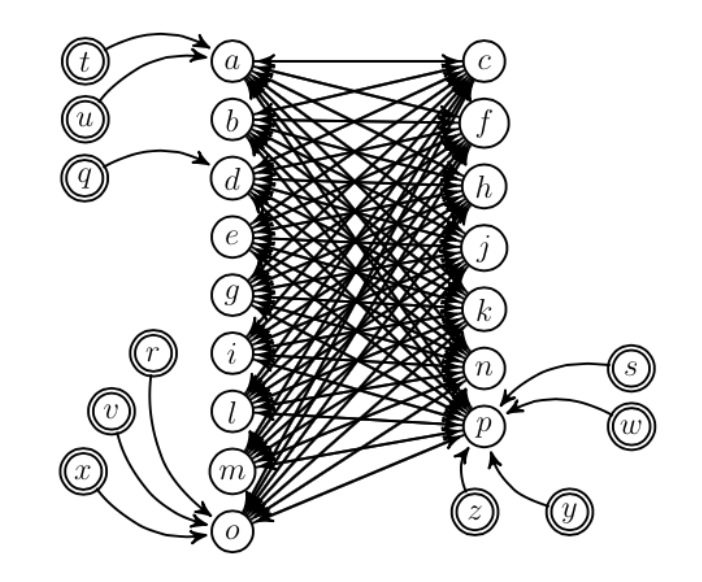
\includegraphics[width=0.5\textwidth]{argumentationframework}
\end{figure}

He modelled this interaction mathematically as a directed graph; with nodes representing the arguments and edges representing the attack relations between the arguments. This model of arguments and attack relations is known as an argumentation framework.

Within an argumentation framework an argument A can become inadmissible if it is attacked by another argument B. However, if B is attacked by C and becomes in admissible then A may be reinstated.

\begin{figure}[h]
\caption{A is reinstated since C attacks B}
\centering
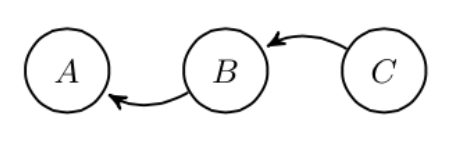
\includegraphics[width=0.5\textwidth]{defeatrelations}
\end{figure}

\subsection{Semantics}

\subsection{Argumentation Theory Implementations}

Prakken and Modgil (2013) presented a tutorial introduction to ASPIC+; a framework for structured argumentation that is meant to generate abstract argumentation frameworks similar to those described by Dung. Within their framework arguments could be attacked in three ways: their uncertain premises, their defeasible inferences or on the conclusions of their defeasible inferences. The authors claim that Dungs calculus is indispensable, it provides little guidance for the modelling of such a system. ASPIC+ is proposed as a framework to guide the implementation of such a system, but is not itself implemented.

Computers can be used to model arguments using visualisation techniques. An example of this is argument diagramming tools; effective aids in helping people reason about arguments. Araucaria is one such tool is described by Reed and Rowe (2001). Araucaria was designed to make argument diagramming for undergraduates easier and also to support research activities. Reed and Rowe also developed AML (Argument Markup Language) an XML based syntax for describing the structure of arguments. Unlike Dung’s argumentation framework, Araucaria represents arguments in a tree structure and the branches of this tree represent support relations as opposed to defeat relations.

Implementations of argumentation systems are more commonly based around decision support systems. A review of defeasible reasoning implementations by Bryant and Krause (2004) highlight the need for well designed empirical evaluations of implementations and formal complexity analysis to justify the practical applicability of a reasoning engine. The paper also highlights the proprietary nature of successful argumentation theory based applications preventing researchers from peer reviewing the software.

Karacapilidis and Papadias (2001) describe HERMES, a system for computer supported argumentation and decision making. HERMES also provides users with access to information from external databases to further justify their arguments. Arguments are represented using a labelling approach as opposed to a graph approach. Constraints are inserted into a discussion graph and when new constraints are introduced they are checked against existing ones.

The fact that decision support systems allow users to aggregate evidence and make decisions based on that evidence lends makes them an obvious fit for medical practitioners. Hunter and Williams (2010) developed a framework for generating inference rules to argue for and against the benefits of medical treatments based on evidence. Their work highlights the benefits of argumentation systems in abstracting away the complicated nature of medical evidence into a form more manageable for practitioners.

Longo and Hederman (2013) similarly investigated the role of argumentation theory in the implementation of decision support systems. Their work provides a comparison with machine learning. The authors developed an argumentation framework (similar to to those described by Dung) to model the breast cancer recurrence problem. The results of their experiment showed that argumentation based systems could perform as well and in some cases better than machine learning algorithms.


%----------------------------------------------------------------------------------------
%	CONCLUSIONS
%----------------------------------------------------------------------------------------

\section{Conclusions}
